\documentclass[11pt,compress,t,notes=noshow, xcolor=table]{beamer}
\usepackage[]{graphicx}
\usepackage[]{color}
% maxwidth is the original width if it is less than linewidth
% otherwise use linewidth (to make sure the graphics do not exceed the margin)
\makeatletter
\def\maxwidth{ %
  \ifdim\Gin@nat@width>\linewidth
    \linewidth
  \else
    \Gin@nat@width
  \fi
}
\makeatother

% ---------------------------------%
% latex-math dependencies, do not remove:
% - \usepackage{mathtools}
% - \usepackage{bm}
% - \usepackage{siunitx}
% - \usepackage{dsfont}
% - \usepackage{xspace}
% ---------------------------------%

%--------------------------------------------------------%
%       Language, encoding, typography
%--------------------------------------------------------%

\usepackage[english]{babel}
\usepackage[utf8]{inputenc} % Enables inputting UTF-8 symbols
% Standard AMS suite
\usepackage{amsmath,amsfonts,amssymb}

% Font four double-stroke / blackboard letters for sets of numbers (N, R, ...)
% Distribution name is "doublestroke"
% According to https://mirror.physik.tu-berlin.de/pub/CTAN/fonts/doublestroke/dsdoc.pdf
% the "bbm" package does a similar thing and may be superfluous.
% Required for latex-math
\usepackage{dsfont}

% bbm – "Blackboard-style" cm fonts (https://www.ctan.org/pkg/bbm)
% Used to be in common.tex, loaded directly after this file
% Maybe superfluous given dsfont is loaded
% TODO: Check if really unused?
% \usepackage{bbm}

% bm – Access bold symbols in maths mode - https://ctan.org/pkg/bm
% Required for latex-math
% https://tex.stackexchange.com/questions/3238/bm-package-versus-boldsymbol
\usepackage{bm}

% pifont – Access to PostScript standard Symbol and Dingbats fonts
% Used for \newcommand{\xmark}{\ding{55}, which is never used
% aside from lecture_advml/attic/xx-automl/slides.Rnw
% \usepackage{pifont}

% Quotes (inline and display), provdes \enquote
% https://ctan.org/pkg/csquotes
\usepackage{csquotes}

% Adds arg to enumerate env, technically superseded by enumitem according
% to https://ctan.org/pkg/enumerate
% Replace with https://ctan.org/pkg/enumitem ?
\usepackage{enumerate}

% Line spacing - provides \singlespacing \doublespacing \onehalfspacing
% https://ctan.org/pkg/setspace
% TODO: Check if really unused?
%\usepackage{setspace}

% mathtools – Mathematical tools to use with amsmath
% https://ctan.org/pkg/mathtools?lang=en
% latex-math dependency according to latex-math repo
\usepackage{mathtools}

%--------------------------------------------------------%
%       Displaying code and algorithms
%--------------------------------------------------------%
\usepackage{verbatim}
\usepackage{algorithm}
\usepackage{algpseudocode}

%--------------------------------------------------------%
%       Tables
%--------------------------------------------------------%

% multi-row table cells: https://www.namsu.de/Extra/pakete/Multirow.html
\usepackage{multirow}

% long/multi-page tables: https://texdoc.org/serve/longtable.pdf/0
% TODO: Check if really unused?

\usepackage{longtable}

% pretty table env: https://ctan.org/pkg/booktabs?lang=en
% TODO: Check if really unused?
\usepackage{booktabs}

%--------------------------------------------------------%
%       Figures: Creating, placing, verbing
%--------------------------------------------------------%

% wrapfig - Wrapping text around figures https://de.overleaf.com/learn/latex/Wrapping_text_around_figures
\usepackage{wrapfig}

% Sub figures in figures and tables
% https://ctan.org/pkg/subfig -- supersedes subfigure package
% TODO: Check if really unused?
\usepackage{subfig}

% Actually it's pronounced PGF https://en.wikibooks.org/wiki/LaTeX/PGF/TikZ
\usepackage{tikz}

\usetikzlibrary{shapes,arrows,automata,positioning,calc,chains,trees, shadows}
\tikzset{
  %Define standard arrow tip
  >=stealth',
  %Define style for boxes
  punkt/.style={
    rectangle,
    rounded corners,
    draw=black, very thick,
    text width=6.5em,
    minimum height=2em,
    text centered},
  % Define arrow style
  pil/.style={
    ->,
    thick,
    shorten <=2pt,
    shorten >=2pt,}
}


% Unsorted
% textpos – Place boxes at arbitrary positions on the LATEX page
% https://ctan.org/pkg/textpos?lang=en
% Provides \begin{textblock}
 % TODO: Check if really unused?
\usepackage[absolute,overlay]{textpos}

% psfrag – Replace strings in encapsulated PostScript figures
% https://www.overleaf.com/latex/examples/psfrag-example/tggxhgzwrzhn
% https://ftp.mpi-inf.mpg.de/pub/tex/mirror/ftp.dante.de/pub/tex/macros/latex/contrib/psfrag/pfgguide.pdf
% Can't tell if this is needed
% TODO: Check if really unused?
\usepackage{psfrag}

% Maybe not great to use this https://tex.stackexchange.com/a/197/19093
% Use align instead -- TODO: Global search & replace to check
\usepackage{eqnarray}

\usepackage{colortbl}

% arydshln – Draw dash-lines in array/tabular
% https://www.ctan.org/pkg/arydshln
% !! "arydshln has to be loaded after array, longtable, colortab and/or colortbl"
% Provides \hdashline and \cdashline
% TODO: Check if really unused?
% \usepackage{arydshln}

% tabularx – Tabulars with adjustable-width columns
% https://ctan.org/pkg/tabularx
% Provides \begin{tabularx}
% TODO: Check if really unused?
% \usepackage{tabularx}

% placeins – Control float placement
% https://ctan.org/pkg/placeins
% Defines a \FloatBarrier command
% TODO: Check if really unused?
% \usepackage{placeins}


% framed – Framed or shaded regions that can break across pages
% https://ctan.org/pkg/framed
% Provides \begin{framed} which uses \colorbox{shadecolor} relying on \definecolor{shadecolor}.
% TODO: Check if really unused?
% \usepackage{framed}

% Used often in conjunction with \definecolor{shadecolor}{rgb}{0.969, 0.969, 0.969}
% Might be able to be removed or at least redefined to only have shadecolor (if needed)
\definecolor{fgcolor}{rgb}{0.345, 0.345, 0.345}
\definecolor{shadecolor}{rgb}{0.969, 0.969, 0.969}
\newenvironment{knitrout}{}{} % an empty environment to be redefined in TeX


% Defines macros and environments
\usepackage{../../style/lmu-lecture}

\let\code=\texttt % Used regularly
\let\proglang=\textsf % Unused?

% Not sure what/why this does
\setkeys{Gin}{width=0.9\textwidth}

\setbeamertemplate{frametitle}{\expandafter\uppercase\expandafter\insertframetitle}

% Can't find a reason why common.tex is not just part of this file?
% Rarely used fontstyle for R packages, used only in 
% - forests/slides-forests-benchmark.tex
% - exercises/single-exercises/methods_l_1.Rnw
% - slides/cart/attic/slides_extra_trees.Rnw
\newcommand{\pkg}[1]{{\fontseries{b}\selectfont #1}}

% Spacing helpers, used often (mostly in exercises for \dlz)
\newcommand{\lz}{\vspace{0.5cm}} % vertical space (used often in slides)
\newcommand{\dlz}{\vspace{1cm}}  % double vertical space (used often in exercises, never in slides)

%--------------------%
%  New environments  %
%--------------------%

 % Frame with breaks and verbatim // this is used very often
\newenvironment{vbframe}
{
\begin{frame}[containsverbatim,allowframebreaks]
}
{
\end{frame}
}

% Frame with verbatim without breaks (to avoid numbering one slided frames)
% This is not used anywhere but I can see it being useful
\newenvironment{vframe}
{
\begin{frame}[containsverbatim]
}
{
\end{frame}
}

% Itemize block
\newenvironment{blocki}[1]
{
\begin{block}{#1}\begin{itemize}
}
{
\end{itemize}\end{block}
}

% textcolor that works in mathmode
% https://tex.stackexchange.com/a/261480
% Used e.g. in forests/slides-forests-bagging.tex
% [...] \textcolor{blue}{\tfrac{1}{M}\sum^M_{m} [...]
% \makeatletter
% \renewcommand*{\@textcolor}[3]{%
%   \protect\leavevmode
%   \begingroup
%     \color#1{#2}#3%
%   \endgroup
% }
% \makeatother


%-------------------------------------------------------------------------------------------------------%
%  Unused stuff that needs to go but is kept here currently juuuust in case it was important after all  %
%-------------------------------------------------------------------------------------------------------%

% \newcommand{\hlnum}[1]{\textcolor[rgb]{0.686,0.059,0.569}{#1}}%
% \newcommand{\hlstr}[1]{\textcolor[rgb]{0.192,0.494,0.8}{#1}}%
% \newcommand{\hlcom}[1]{\textcolor[rgb]{0.678,0.584,0.686}{\textit{#1}}}%
% \newcommand{\hlopt}[1]{\textcolor[rgb]{0,0,0}{#1}}%
% \newcommand{\hlstd}[1]{\textcolor[rgb]{0.345,0.345,0.345}{#1}}%
% \newcommand{\hlkwa}[1]{\textcolor[rgb]{0.161,0.373,0.58}{\textbf{#1}}}%
% \newcommand{\hlkwb}[1]{\textcolor[rgb]{0.69,0.353,0.396}{#1}}%
% \newcommand{\hlkwc}[1]{\textcolor[rgb]{0.333,0.667,0.333}{#1}}%
% \newcommand{\hlkwd}[1]{\textcolor[rgb]{0.737,0.353,0.396}{\textbf{#1}}}%
% \let\hlipl\hlkwb

% \makeatletter
% \newenvironment{kframe}{%
%  \def\at@end@of@kframe{}%
%  \ifinner\ifhmode%
%   \def\at@end@of@kframe{\end{minipage}}%
%   \begin{minipage}{\columnwidth}%
%  \fi\fi%
%  \def\FrameCommand##1{\hskip\@totalleftmargin \hskip-\fboxsep
%  \colorbox{shadecolor}{##1}\hskip-\fboxsep
%      % There is no \\@totalrightmargin, so:
%      \hskip-\linewidth \hskip-\@totalleftmargin \hskip\columnwidth}%
%  \MakeFramed {\advance\hsize-\width
%    \@totalleftmargin\z@ \linewidth\hsize
%    \@setminipage}}%
%  {\par\unskip\endMakeFramed%
%  \at@end@of@kframe}
% \makeatother

% \definecolor{shadecolor}{rgb}{.97, .97, .97}
% \definecolor{messagecolor}{rgb}{0, 0, 0}
% \definecolor{warningcolor}{rgb}{1, 0, 1}
% \definecolor{errorcolor}{rgb}{1, 0, 0}
% \newenvironment{knitrout}{}{} % an empty environment to be redefined in TeX

% \usepackage{alltt}
% \newcommand{\SweaveOpts}[1]{}  % do not interfere with LaTeX
% \newcommand{\SweaveInput}[1]{} % because they are not real TeX commands
% \newcommand{\Sexpr}[1]{}       % will only be parsed by R
% \newcommand{\xmark}{\ding{55}}%

% dependencies: amsmath, amssymb, dsfont
% math spaces
\ifdefined\N
\renewcommand{\N}{\mathds{N}} % N, naturals
\else \newcommand{\N}{\mathds{N}} \fi
\newcommand{\Z}{\mathds{Z}} % Z, integers
\newcommand{\Q}{\mathds{Q}} % Q, rationals
\newcommand{\R}{\mathds{R}} % R, reals
\ifdefined\C
\renewcommand{\C}{\mathds{C}} % C, complex
\else \newcommand{\C}{\mathds{C}} \fi
\newcommand{\continuous}{\mathcal{C}} % C, space of continuous functions
\newcommand{\M}{\mathcal{M}} % machine numbers
\newcommand{\epsm}{\epsilon_m} % maximum error

% counting / finite sets
\newcommand{\setzo}{\{0, 1\}} % set 0, 1
\newcommand{\setmp}{\{-1, +1\}} % set -1, 1
\newcommand{\unitint}{[0, 1]} % unit interval

% basic math stuff
\newcommand{\xt}{\tilde x} % x tilde
\DeclareMathOperator*{\argmax}{arg\,max} % argmax
\DeclareMathOperator*{\argmin}{arg\,min} % argmin
\newcommand{\argminlim}{\mathop{\mathrm{arg\,min}}\limits} % argmax with limits
\newcommand{\argmaxlim}{\mathop{\mathrm{arg\,max}}\limits} % argmin with limits
\newcommand{\sign}{\operatorname{sign}} % sign, signum
\newcommand{\I}{\mathbb{I}} % I, indicator
\newcommand{\order}{\mathcal{O}} % O, order
\newcommand{\bigO}{\mathcal{O}} % Big-O Landau
\newcommand{\littleo}{{o}} % Little-o Landau
\newcommand{\pd}[2]{\frac{\partial{#1}}{\partial #2}} % partial derivative
\newcommand{\floorlr}[1]{\left\lfloor #1 \right\rfloor} % floor
\newcommand{\ceillr}[1]{\left\lceil #1 \right\rceil} % ceiling
\newcommand{\indep}{\perp \!\!\! \perp} % independence symbol

% sums and products
\newcommand{\sumin}{\sum\limits_{i=1}^n} % summation from i=1 to n
\newcommand{\sumim}{\sum\limits_{i=1}^m} % summation from i=1 to m
\newcommand{\sumjn}{\sum\limits_{j=1}^n} % summation from j=1 to p
\newcommand{\sumjp}{\sum\limits_{j=1}^p} % summation from j=1 to p
\newcommand{\sumik}{\sum\limits_{i=1}^k} % summation from i=1 to k
\newcommand{\sumkg}{\sum\limits_{k=1}^g} % summation from k=1 to g
\newcommand{\sumjg}{\sum\limits_{j=1}^g} % summation from j=1 to g
\newcommand{\meanin}{\frac{1}{n} \sum\limits_{i=1}^n} % mean from i=1 to n
\newcommand{\meanim}{\frac{1}{m} \sum\limits_{i=1}^m} % mean from i=1 to n
\newcommand{\meankg}{\frac{1}{g} \sum\limits_{k=1}^g} % mean from k=1 to g
\newcommand{\prodin}{\prod\limits_{i=1}^n} % product from i=1 to n
\newcommand{\prodkg}{\prod\limits_{k=1}^g} % product from k=1 to g
\newcommand{\prodjp}{\prod\limits_{j=1}^p} % product from j=1 to p

% linear algebra
\newcommand{\one}{\bm{1}} % 1, unitvector
\newcommand{\zero}{\mathbf{0}} % 0-vector
\newcommand{\id}{\bm{I}} % I, identity
\newcommand{\diag}{\operatorname{diag}} % diag, diagonal
\newcommand{\trace}{\operatorname{tr}} % tr, trace
\newcommand{\spn}{\operatorname{span}} % span
\newcommand{\scp}[2]{\left\langle #1, #2 \right\rangle} % <.,.>, scalarproduct
\newcommand{\mat}[1]{\begin{pmatrix} #1 \end{pmatrix}} % short pmatrix command
\newcommand{\Amat}{\mathbf{A}} % matrix A
\newcommand{\Deltab}{\mathbf{\Delta}} % error term for vectors

% basic probability + stats
\renewcommand{\P}{\mathds{P}} % P, probability
\newcommand{\E}{\mathds{E}} % E, expectation
\newcommand{\var}{\mathsf{Var}} % Var, variance
\newcommand{\cov}{\mathsf{Cov}} % Cov, covariance
\newcommand{\corr}{\mathsf{Corr}} % Corr, correlation
\newcommand{\normal}{\mathcal{N}} % N of the normal distribution
\newcommand{\iid}{\overset{i.i.d}{\sim}} % dist with i.i.d superscript
\newcommand{\distas}[1]{\overset{#1}{\sim}} % ... is distributed as ...

% machine learning
\newcommand{\Xspace}{\mathcal{X}} % X, input space
\newcommand{\Yspace}{\mathcal{Y}} % Y, output space
\newcommand{\Zspace}{\mathcal{Z}} % Space of sampled datapoints ! Also defined identically in ml-online.tex !
\newcommand{\nset}{\{1, \ldots, n\}} % set from 1 to n
\newcommand{\pset}{\{1, \ldots, p\}} % set from 1 to p
\newcommand{\gset}{\{1, \ldots, g\}} % set from 1 to g
\newcommand{\Pxy}{\mathbb{P}_{xy}} % P_xy
\newcommand{\Exy}{\mathbb{E}_{xy}} % E_xy: Expectation over random variables xy
\newcommand{\xv}{\mathbf{x}} % vector x (bold)
\newcommand{\xtil}{\tilde{\mathbf{x}}} % vector x-tilde (bold)
\newcommand{\yv}{\mathbf{y}} % vector y (bold)
\newcommand{\xy}{(\xv, y)} % observation (x, y)
\newcommand{\xvec}{\left(x_1, \ldots, x_p\right)^\top} % (x1, ..., xp)
\newcommand{\Xmat}{\mathbf{X}} % Design matrix
\newcommand{\allDatasets}{\mathds{D}} % The set of all datasets
\newcommand{\allDatasetsn}{\mathds{D}_n}  % The set of all datasets of size n
\newcommand{\D}{\mathcal{D}} % D, data
\newcommand{\Dn}{\D_n} % D_n, data of size n
\newcommand{\Dtrain}{\mathcal{D}_{\text{train}}} % D_train, training set
\newcommand{\Dtest}{\mathcal{D}_{\text{test}}} % D_test, test set
\newcommand{\xyi}[1][i]{\left(\xv^{(#1)}, y^{(#1)}\right)} % (x^i, y^i), i-th observation
\newcommand{\Dset}{\left( \xyi[1], \ldots, \xyi[n]\right)} % {(x1,y1)), ..., (xn,yn)}, data
\newcommand{\defAllDatasetsn}{(\Xspace \times \Yspace)^n} % Def. of the set of all datasets of size n
\newcommand{\defAllDatasets}{\bigcup_{n \in \N}(\Xspace \times \Yspace)^n} % Def. of the set of all datasets
\newcommand{\xdat}{\left\{ \xv^{(1)}, \ldots, \xv^{(n)}\right\}} % {x1, ..., xn}, input data
\newcommand{\ydat}{\left\{ \yv^{(1)}, \ldots, \yv^{(n)}\right\}} % {y1, ..., yn}, input data
\newcommand{\yvec}{\left(y^{(1)}, \hdots, y^{(n)}\right)^\top} % (y1, ..., yn), vector of outcomes
\renewcommand{\xi}[1][i]{\xv^{(#1)}} % x^i, i-th observed value of x
\newcommand{\yi}[1][i]{y^{(#1)}} % y^i, i-th observed value of y
\newcommand{\xivec}{\left(x^{(i)}_1, \ldots, x^{(i)}_p\right)^\top} % (x1^i, ..., xp^i), i-th observation vector
\newcommand{\xj}{\xv_j} % x_j, j-th feature
\newcommand{\xjvec}{\left(x^{(1)}_j, \ldots, x^{(n)}_j\right)^\top} % (x^1_j, ..., x^n_j), j-th feature vector
\newcommand{\phiv}{\mathbf{\phi}} % Basis transformation function phi
\newcommand{\phixi}{\mathbf{\phi}^{(i)}} % Basis transformation of xi: phi^i := phi(xi)

%%%%%% ml - models general
\newcommand{\lamv}{\bm{\lambda}} % lambda vector, hyperconfiguration vector
\newcommand{\Lam}{\bm{\Lambda}}	 % Lambda, space of all hpos
% Inducer / Inducing algorithm
\newcommand{\preimageInducer}{\left(\defAllDatasets\right)\times\Lam} % Set of all datasets times the hyperparameter space
\newcommand{\preimageInducerShort}{\allDatasets\times\Lam} % Set of all datasets times the hyperparameter space
% Inducer / Inducing algorithm
\newcommand{\ind}{\mathcal{I}} % Inducer, inducing algorithm, learning algorithm

% continuous prediction function f
\newcommand{\ftrue}{f_{\text{true}}}  % True underlying function (if a statistical model is assumed)
\newcommand{\ftruex}{\ftrue(\xv)} % True underlying function (if a statistical model is assumed)
\newcommand{\fx}{f(\xv)} % f(x), continuous prediction function
\newcommand{\fdomains}{f: \Xspace \rightarrow \R^g} % f with domain and co-domain
\newcommand{\Hspace}{\mathcal{H}} % hypothesis space where f is from
\newcommand{\fbayes}{f^{\ast}} % Bayes-optimal model
\newcommand{\fxbayes}{f^{\ast}(\xv)} % Bayes-optimal model
\newcommand{\fkx}[1][k]{f_{#1}(\xv)} % f_j(x), discriminant component function
\newcommand{\fh}{\hat{f}} % f hat, estimated prediction function
\newcommand{\fxh}{\fh(\xv)} % fhat(x)
\newcommand{\fxt}{f(\xv ~|~ \thetab)} % f(x | theta)
\newcommand{\fxi}{f\left(\xv^{(i)}\right)} % f(x^(i))
\newcommand{\fxih}{\hat{f}\left(\xv^{(i)}\right)} % f(x^(i))
\newcommand{\fxit}{f\left(\xv^{(i)} ~|~ \thetab\right)} % f(x^(i) | theta)
\newcommand{\fhD}{\fh_{\D}} % fhat_D, estimate of f based on D
\newcommand{\fhDtrain}{\fh_{\Dtrain}} % fhat_Dtrain, estimate of f based on D
\newcommand{\fhDnlam}{\fh_{\Dn, \lamv}} %model learned on Dn with hp lambda
\newcommand{\fhDlam}{\fh_{\D, \lamv}} %model learned on D with hp lambda
\newcommand{\fhDnlams}{\fh_{\Dn, \lamv^\ast}} %model learned on Dn with optimal hp lambda
\newcommand{\fhDlams}{\fh_{\D, \lamv^\ast}} %model learned on D with optimal hp lambda

% discrete prediction function h
\newcommand{\hx}{h(\xv)} % h(x), discrete prediction function
\newcommand{\hh}{\hat{h}} % h hat
\newcommand{\hxh}{\hat{h}(\xv)} % hhat(x)
\newcommand{\hxt}{h(\xv | \thetab)} % h(x | theta)
\newcommand{\hxi}{h\left(\xi\right)} % h(x^(i))
\newcommand{\hxit}{h\left(\xi ~|~ \thetab\right)} % h(x^(i) | theta)
\newcommand{\hbayes}{h^{\ast}} % Bayes-optimal classification model
\newcommand{\hxbayes}{h^{\ast}(\xv)} % Bayes-optimal classification model

% yhat
\newcommand{\yh}{\hat{y}} % yhat for prediction of target
\newcommand{\yih}{\hat{y}^{(i)}} % yhat^(i) for prediction of ith targiet
\newcommand{\resi}{\yi- \yih}

% theta
\newcommand{\thetah}{\hat{\theta}} % theta hat
\newcommand{\thetab}{\bm{\theta}} % theta vector
\newcommand{\thetabh}{\bm{\hat\theta}} % theta vector hat
\newcommand{\thetat}[1][t]{\thetab^{[#1]}} % theta^[t] in optimization
\newcommand{\thetatn}[1][t]{\thetab^{[#1 +1]}} % theta^[t+1] in optimization
\newcommand{\thetahDnlam}{\thetabh_{\Dn, \lamv}} %theta learned on Dn with hp lambda
\newcommand{\thetahDlam}{\thetabh_{\D, \lamv}} %theta learned on D with hp lambda
\newcommand{\mint}{\min_{\thetab \in \Theta}} % min problem theta
\newcommand{\argmint}{\argmin_{\thetab \in \Theta}} % argmin theta

% densities + probabilities
% pdf of x
\newcommand{\pdf}{p} % p
\newcommand{\pdfx}{p(\xv)} % p(x)
\newcommand{\pixt}{\pi(\xv~|~ \thetab)} % pi(x|theta), pdf of x given theta
\newcommand{\pixit}[1][i]{\pi\left(\xi[#1] ~|~ \thetab\right)} % pi(x^i|theta), pdf of x given theta
\newcommand{\pixii}[1][i]{\pi\left(\xi[#1]\right)} % pi(x^i), pdf of i-th x

% pdf of (x, y)
\newcommand{\pdfxy}{p(\xv,y)} % p(x, y)
\newcommand{\pdfxyt}{p(\xv, y ~|~ \thetab)} % p(x, y | theta)
\newcommand{\pdfxyit}{p\left(\xi, \yi ~|~ \thetab\right)} % p(x^(i), y^(i) | theta)

% pdf of x given y
\newcommand{\pdfxyk}[1][k]{p(\xv | y= #1)} % p(x | y = k)
\newcommand{\lpdfxyk}[1][k]{\log p(\xv | y= #1)} % log p(x | y = k)
\newcommand{\pdfxiyk}[1][k]{p\left(\xi | y= #1 \right)} % p(x^i | y = k)

% prior probabilities
\newcommand{\pik}[1][k]{\pi_{#1}} % pi_k, prior
\newcommand{\lpik}[1][k]{\log \pi_{#1}} % log pi_k, log of the prior
\newcommand{\pit}{\pi(\thetab)} % Prior probability of parameter theta

% posterior probabilities
\newcommand{\post}{\P(y = 1 ~|~ \xv)} % P(y = 1 | x), post. prob for y=1
\newcommand{\postk}[1][k]{\P(y = #1 ~|~ \xv)} % P(y = k | y), post. prob for y=k
\newcommand{\pidomains}{\pi: \Xspace \rightarrow \unitint} % pi with domain and co-domain
\newcommand{\pibayes}{\pi^{\ast}} % Bayes-optimal classification model
\newcommand{\pixbayes}{\pi^{\ast}(\xv)} % Bayes-optimal classification model
\newcommand{\pix}{\pi(\xv)} % pi(x), P(y = 1 | x)
\newcommand{\piv}{\bm{\pi}} % pi, bold, as vector
\newcommand{\pikx}[1][k]{\pi_{#1}(\xv)} % pi_k(x), P(y = k | x)
\newcommand{\pikxt}[1][k]{\pi_{#1}(\xv ~|~ \thetab)} % pi_k(x | theta), P(y = k | x, theta)
\newcommand{\pixh}{\hat \pi(\xv)} % pi(x) hat, P(y = 1 | x) hat
\newcommand{\pikxh}[1][k]{\hat \pi_{#1}(\xv)} % pi_k(x) hat, P(y = k | x) hat
\newcommand{\pixih}{\hat \pi(\xi)} % pi(x^(i)) with hat
\newcommand{\pikxih}[1][k]{\hat \pi_{#1}(\xi)} % pi_k(x^(i)) with hat
\newcommand{\pdfygxt}{p(y ~|~\xv, \thetab)} % p(y | x, theta)
\newcommand{\pdfyigxit}{p\left(\yi ~|~\xi, \thetab\right)} % p(y^i |x^i, theta)
\newcommand{\lpdfygxt}{\log \pdfygxt } % log p(y | x, theta)
\newcommand{\lpdfyigxit}{\log \pdfyigxit} % log p(y^i |x^i, theta)

% probababilistic
\newcommand{\bayesrulek}[1][k]{\frac{\P(\xv | y= #1) \P(y= #1)}{\P(\xv)}} % Bayes rule
\newcommand{\muk}{\bm{\mu_k}} % mean vector of class-k Gaussian (discr analysis)

% residual and margin
\newcommand{\eps}{\epsilon} % residual, stochastic
\newcommand{\epsi}{\epsilon^{(i)}} % epsilon^i, residual, stochastic
\newcommand{\epsh}{\hat{\epsilon}} % residual, estimated
\newcommand{\yf}{y \fx} % y f(x), margin
\newcommand{\yfi}{\yi \fxi} % y^i f(x^i), margin
\newcommand{\Sigmah}{\hat \Sigma} % estimated covariance matrix
\newcommand{\Sigmahj}{\hat \Sigma_j} % estimated covariance matrix for the j-th class

% ml - loss, risk, likelihood
\newcommand{\Lyf}{L\left(y, f\right)} % L(y, f), loss function
\newcommand{\Lypi}{L\left(y, \pi\right)} % L(y, pi), loss function
\newcommand{\Lxy}{L\left(y, \fx\right)} % L(y, f(x)), loss function
\newcommand{\Lxyi}{L\left(\yi, \fxi\right)} % loss of observation
\newcommand{\Lxyt}{L\left(y, \fxt\right)} % loss with f parameterized
\newcommand{\Lxyit}{L\left(\yi, \fxit\right)} % loss of observation with f parameterized
\newcommand{\Lxym}{L\left(\yi, f\left(\bm{\tilde{x}}^{(i)} ~|~ \thetab\right)\right)} % loss of observation with f parameterized
\newcommand{\Lpixy}{L\left(y, \pix\right)} % loss in classification
\newcommand{\Lpiv}{L\left(y, \piv\right)} % loss in classification
\newcommand{\Lpixyi}{L\left(\yi, \pixii\right)} % loss of observation in classification
\newcommand{\Lpixyt}{L\left(y, \pixt\right)} % loss with pi parameterized
\newcommand{\Lpixyit}{L\left(\yi, \pixit\right)} % loss of observation with pi parameterized
\newcommand{\Lhxy}{L\left(y, \hx\right)} % L(y, h(x)), loss function on discrete classes
\newcommand{\Lr}{L\left(r\right)} % L(r), loss defined on residual (reg) / margin (classif)
\newcommand{\lone}{|y - \fx|} % L1 loss
\newcommand{\ltwo}{\left(y - \fx\right)^2} % L2 loss
\newcommand{\lbernoullimp}{\ln(1 + \exp(-y \cdot \fx))} % Bernoulli loss for -1, +1 encoding
\newcommand{\lbernoullizo}{- y \cdot \fx + \log(1 + \exp(\fx))} % Bernoulli loss for 0, 1 encoding
\newcommand{\lcrossent}{- y \log \left(\pix\right) - (1 - y) \log \left(1 - \pix\right)} % cross-entropy loss
\newcommand{\lbrier}{\left(\pix - y \right)^2} % Brier score
\newcommand{\risk}{\mathcal{R}} % R, risk
\newcommand{\riskbayes}{\mathcal{R}^\ast}
\newcommand{\riskf}{\risk(f)} % R(f), risk
\newcommand{\riskdef}{\E_{y|\xv}\left(\Lxy \right)} % risk def (expected loss)
\newcommand{\riskt}{\mathcal{R}(\thetab)} % R(theta), risk
\newcommand{\riske}{\mathcal{R}_{\text{emp}}} % R_emp, empirical risk w/o factor 1 / n
\newcommand{\riskeb}{\bar{\mathcal{R}}_{\text{emp}}} % R_emp, empirical risk w/ factor 1 / n
\newcommand{\riskef}{\riske(f)} % R_emp(f)
\newcommand{\risket}{\mathcal{R}_{\text{emp}}(\thetab)} % R_emp(theta)
\newcommand{\riskr}{\mathcal{R}_{\text{reg}}} % R_reg, regularized risk
\newcommand{\riskrt}{\mathcal{R}_{\text{reg}}(\thetab)} % R_reg(theta)
\newcommand{\riskrf}{\riskr(f)} % R_reg(f)
\newcommand{\riskrth}{\hat{\mathcal{R}}_{\text{reg}}(\thetab)} % hat R_reg(theta)
\newcommand{\risketh}{\hat{\mathcal{R}}_{\text{emp}}(\thetab)} % hat R_emp(theta)
\newcommand{\LL}{\mathcal{L}} % L, likelihood
\newcommand{\LLt}{\mathcal{L}(\thetab)} % L(theta), likelihood
\newcommand{\LLtx}{\mathcal{L}(\thetab | \xv)} % L(theta|x), likelihood
\newcommand{\logl}{\ell} % l, log-likelihood
\newcommand{\loglt}{\logl(\thetab)} % l(theta), log-likelihood
\newcommand{\logltx}{\logl(\thetab | \xv)} % l(theta|x), log-likelihood
\newcommand{\errtrain}{\text{err}_{\text{train}}} % training error
\newcommand{\errtest}{\text{err}_{\text{test}}} % test error
\newcommand{\errexp}{\overline{\text{err}_{\text{test}}}} % avg training error

% lm
\newcommand{\thx}{\thetab^\top \xv} % linear model
\newcommand{\olsest}{(\Xmat^\top \Xmat)^{-1} \Xmat^\top \yv} % OLS estimator in LM


%\usepackage{algorithm}
%\usepackage{algorithmic}

\newcommand{\sens}{\mathbf{A}} % vector x (bold)
\newcommand{\ba}{\mathbf{a}}
\newcommand{\batilde}{\tilde{\mathbf{a}}}
\newcommand{\Px}{\mathbb{P}_{x}} % P_x
\newcommand{\Pxj}{\mathbb{P}_{x_j}} % P_{x_j}
\newcommand{\indep}{\perp \!\!\! \perp} % independence symbol
% ml - ROC
\newcommand{\np}{n_{+}} % no. of positive instances
\newcommand{\nn}{n_{-}} % no. of negative instances
\newcommand{\rn}{\pi_{-}} % proportion negative instances
\newcommand{\rp}{\pi_{+}} % proportion negative instances
% true/false pos/neg:
\newcommand{\tp}{\# \text{TP}} % true pos
\newcommand{\fap}{\# \text{FP}} % false pos (fp taken for partial derivs)
\newcommand{\tn}{\# \text{TN}} % true neg
\newcommand{\fan}{\# \text{FN}} % false neg

\usepackage{multicol}

\newcommand{\titlefigure}{figure/cost_matrix}
\newcommand{\learninggoals}{
  \item Learn cost matrix modelling in cost-sensitive learning
  \item Understand Minimum Expected Cost Principle
  \item Learn threshold adjusting in cost-sensitive learning
  \item Get to know MetaCost as a general approach to make classifiers cost-sensitve
}

\title{Advanced Machine Learning}
\date{}

\begin{document}

\lecturechapter{Imbalanced Learning via Cost-Sensitive Learning}
\lecture{Advanced Machine Learning}



\sloppy


\begin{vbframe}{Cost-Sensitive learning: In a Nutshell}
	%	
	\scriptsize{
		%
		%
		\begin{itemize}
%			
		\item Cost-sensitive learning: 
            \begin{itemize}
                \scriptsize
                \item Different (mis-)classification costs are taken into consideration.
                \item The learner seeks to minimize the total costs in expectation.
            \end{itemize}
%
		\item Difference to the ``classical'' cost-insensitive learning: 
            \begin{itemize}
                \scriptsize
                \item Cost-sensitive learning deals differently with misclassifications.
                \item Classical learning assumes that the data sets are balanced, and all errors have the same cost.
            \end{itemize}
		
%
		\item Real-world applications, where different costs between misclassifications are present:
%		
		\begin{itemize}
			\scriptsize
%			
			\item Medicine --- Misdiagnosing a cancer patient as healthy vs.\ misdiagnosing a healthy patient as having cancer (and then check again).
			%					
			\item Tracking criminals ---  Classify an innocent person as a terrorist vs.\ overlooking a terrorist.
			%			
			\item (Extreme) Weather prediction ---  Incorrectly predicting that no hurricane occurs vs.\ predicting a strong wind as a hurricane.
%			
			\item Credit granting --- Lending to a risky client vs. not lending to a trustworthy client.
			%			
			\item $\ldots$
%    	
%			
		\end{itemize}
%	
		\item In all these examples, \textbf{the costs of a false negative is much higher than the costs of a false positive}.
%
		\end{itemize}
		
	%
	}
\end{vbframe}


\begin{vbframe}{Cost matrix}
%	
\scriptsize{
%	
	\begin{itemize}
%		
		\item In cost-sensitive learning we are provided with a cost matrix $\mathbf{C}$ of the form
%		
	\end{itemize}
	%	
	\begin{center}
		\tiny
		\begin{tabular}{cc|>{\centering\arraybackslash}p{8em}>{\centering\arraybackslash}p{8em}>{\centering\arraybackslash}p{5em}>{\centering\arraybackslash}p{8em}}
			& & \multicolumn{4}{c}{\bfseries True Class $y$} \\
			&  & $1$ & $2$ & $\ldots$ & $g$  \\
			\hline
			\bfseries Classification     & $1$ & $C(1,1)$  &  $C(1,2)$  & $\ldots$ &  $C(1,g)$ \\
			& $2$ &  $C(2,1)$  &  $C(2,2)$  & $\ldots$ & $C(2,g)$  \\
            $\yh$ & & & & & \\
			& $\vdots$ & $\vdots$ & $\vdots$ & $\ldots$ & $\vdots$ \\
			& $g$ & $C(g,1)$ & $C(g,2)$  & $\ldots$ &  $C(g,g)$\\
		\end{tabular}
	\end{center}
	%	
	\begin{itemize}
		%		
		\item $C(i,j)$ is the cost of classifying $j$ as $i,$ which in the cost-insensitive learning case is simply $C(i,j) = \mathds{1}_{[ i \neq j ]},$ i.e., each misclassification has the same cost of 1.
		\vspace{10pt}
		
		\item Cost matrix is usually designed by using a heuristic or by learning a proper cost matrix from the training data.
        \vspace{10pt}
		\begin{enumerate}
			\scriptsize	
            \item Too low costs: might not change the decision boundaries significantly, leading to (still) costly predictions.
            \vspace{10pt}
            \item Too high costs: might harm the generalization capability of the classifier on costly classes.
            \vspace{10pt}
		\end{enumerate}
		
	\end{itemize}

}
\end{vbframe}


\begin{vbframe}{Cost matrix for Imbalanced Learning}
	\footnotesize{
		\begin{itemize}			
	 
			\item A common heuristic for imbalanced data sets is to use 
	
			\begin{itemize}
				\footnotesize 
                \item $C(i,j) = \frac{n_i}{n_j}$ for classes $i$ and $j$ such that $n_j  \ll n_i$, i.e. for misclassifying a minority class $j$ as a majority class $i$.
                \vspace{10pt}
		
				\item $C(i,j) = 1$ for classes $i$ and $j$ such that $n_i \ll n_j$, i.e. for misclassifying a majority class $j$ as a minority class $i$.
                \vspace{10pt}
			
				\item 0 for a correct classification (a theoretical reason will be explained later).
                \vspace{10pt}
			
			\end{itemize}

    		\item In an imbalanced binary classification we get: \\
            \begin{table}[]
                \centering
                \begin{tabular}{cc|cc}
                    & &\multicolumn{2}{c}{True class} \\
                    & & $y=1$ & $y=-1$  \\
                    \hline
                    \multirow{2}{*}{\parbox{0.3cm}{Pred.  class}}& $\hat y$ = 1     & $0$                & $ 1 $\\
                    & $\hat y$ = -1 & $ \frac{n_-}{n_+} $              &  $0$   \\
                \end{tabular}
            \end{table}
    		

            \item Thus, this heuristic is consistent with the general real case that the cost of false negatives is much higher than the cost of false positives.	
        \end{itemize}
		
	}
\end{vbframe}


\begin{vbframe}{Minimum expected Cost Principle}

	\footnotesize{


		\begin{itemize}\footnotesize
		
			\item Suppose we have:
            \begin{itemize}
                \footnotesize
                \item a cost matrix $\mathbf{C}$,
                \vspace{10pt}
                
                \item knowledge of the true posterior distribution $p(\cdot ~|~ \xv).$
                \vspace{10pt}
            \end{itemize}

            \item Idea for classifying a given feature $\xv$: 
            \begin{itemize}
                \footnotesize
                \item Compute the cost for classifying $\xv$ as $i$. (infeasible to directly compute.)
                \vspace{10pt}
                
                \item $\leadsto$ Marginalize over ``true'' class $j$.
                \vspace{10pt}
            \end{itemize}

			\item \emph{Minimum expected cost principle}: Use the class for prediction with the smallest expected costs, where the expected costs of a class $i\in\{1,\ldots,g\}$ is
	
			$$ 	\E_{J \sim p(\cdot ~|~ \xv)}( C(i,J) ) = \sum_{j=1}^g 	p(j ~|~ \xv) C(i,j).	$$

			
				
		\end{itemize}
	}
\end{vbframe}

\begin{vbframe}{Minimum expected cost principle}
    \footnotesize
    \begin{itemize}
        \item Thus, if we have a classifier $f$ which uses a probabilistic score function $\pi:\Xspace \to [0,1]^g$ with $\pi(\xv) = (\pi(\xv)_1,\ldots,\pi(\xv)_g)^\top$ and $\sum_{j=1}^g \pi(\xv)_j = 1$ for the classification, then one can easily modify $f$ to take the expected costs into account:
		$$  \tilde f (\xv) = \argmin_{i=1,\ldots,g} \sum_{j=1}^g 	\pi(\xv)_j C(i,j). $$
        \vspace{10pt}

        \item For $\xv$, making prediction $i$ means \textbf{acting as if $i$ is the true class of $\xv$.}
        \vspace{10pt}
        
        \item The essence of cost-sensitive decision-making: it can be optimal to act as if class $i$ is true even when $j$ is more probable. (\href{https://dl.acm.org/doi/10.5555/1642194.1642224}{\beamergotobutton{Elkan et. al. 2001}})
        \vspace{10pt}

        \item Now consider: 
        \begin{itemize}
            \footnotesize
            \item If we learnt a binary classifier: $p(1 ~|~ \xv) = \pi(\xv)_1$ and $p(-1 ~|~ \xv) = \pi(\xv)_2$,
            \item Under what condition should we predict $\xv$ as class $1$?
        \end{itemize}
    \end{itemize}
\end{vbframe}


\begin{vbframe}{Minimum expected Cost Principle: Binary Case}
	%	
	\footnotesize{
		%		
		\begin{itemize}
            \footnotesize
            \item Preliminary knowledge: the optimal decisions do NOT change if 
            \begin{itemize}
                \footnotesize
                \item $\mathbf{C}$ is multipled by a positive constant.
                \item $\mathbf{C}$ is added with a constant shift.
            \end{itemize}

            \item Hence, we scale and shift $\mathbf{C}$ to eliminate some entries, obtaining a simpler $\mathbf{C}^\prime$: 
            \begin{table}[]
                \centering
                    \begin{tabular}{cc|cc}
        			& &\multicolumn{2}{c}{True class} \\
        			& & $y=1$ & $y=-1$  \\
        			\hline
        			\multirow{2}{*}{\parbox{0.3cm}{Pred.  class}} & $\hat y$ = 1 & $C^\prime(1,1)$ & $1$ \\
        			& $\hat y$ = -1 & $C^\prime(-1, 1)$ & 0\\
                \end{tabular}
            \end{table}
            where 
            \begin{itemize}
                \footnotesize
                \item $C^\prime (-1, 1) = [C(-1, 1) - C(-1, -1)] / [C(1, -1) - C(-1, -1)]$,
                \item $C^\prime (1, 1) = [C(1, 1) - C(-1, -1)] / [C(1, -1) - C(-1,-1)]$.
            \end{itemize}

            \item We predict $\xv$ as class $1$ if \\
            \begin{align*}
                \E_{J \sim p(\cdot ~|~ \xv)}( C^\prime(1,J) )  \leq \E_{J \sim p(\cdot ~|~ \xv)}( C^\prime(-1,J) ) \\
            \end{align*}

			\item Plugging $\mathbf{C}^\prime$ into the inequality above, we obtain:	
			\begin{align*}	
                & p(-1 ~|~ \xv ) C^\prime(1,-1)  + 	p(1 ~|~ \xv ) C^\prime(1,1) \leq  p(-1 ~|~ \xv ) C^\prime(-1,-1)  + 	p(1 ~|~ \xv ) C^\prime(-1,1)  \\ 
                &\Rightarrow [1 - p(1 ~|~ \xv)] \cdot 1 + p(1 ~|~ \xv) C^\prime(1, 1) \leq p(1 ~|~ \xv) C^\prime(1, -1) \\
                &\Rightarrow p(1 ~|~ \xv) \geq \frac{1}{C^\prime(-1, 1) - C^\prime(1, 1) + 1} \\
                &\Rightarrow p(1 ~|~ \xv) \geq \frac{C(1, -1) - C(-1, -1)}{C(-1, 1) - C(1, 1) + C(1, -1) - C(-1, -1)}
			\end{align*}
		
            \item By further assuming that $C(1, 1) = C(-1, -1) = 0 $, this can by simplied to 
            \begin{align*}
                p(1 ~|~ \xv) \geq \frac{C(1, -1)}{C(-1, 1) + C(1, -1)} = c^{*}
            \end{align*}	
            
            \item This yields the optimal threshold value $c^*$ for probabilistic score classifiers, so that any probabilistic classifier $f$ using a probabilistic score $\pi:\Xspace \to [0,1]$ can be modified to 
            
            $$   \tilde f(\xv) = 2 \cdot \mathds{1}_{[ \pi(\xv) \geq c^*]} -1. $$
							
		\end{itemize}
	}
\end{vbframe}

\begin{vbframe}{Threshold adjusting for imbalanced learning: binary case}
    \footnotesize 
    \begin{itemize}
        \footnotesize
        \item Motivation: The threshold provided by Minimum Expected Cost is sensitive to the choice of $\mathbf{C}$ $\leadsto$ Not always the truly optimal.
        \item Key idea: model the mis-classification cost $M_C$ as a function $M_C = g(T)$ of \textbf{probability threshold} $T \in [0, 1]$.
        \item By adjusting $T$, we can plot a curve of $M_C$ versus $T$ as the following figure (copied from Fig.1 in \href{https://www.aaai.org/Library/AAAI/2006/aaai06-076.php}{\beamergotobutton{Sheng et al. 2006}}):
        \begin{figure}[h]
            \centering
            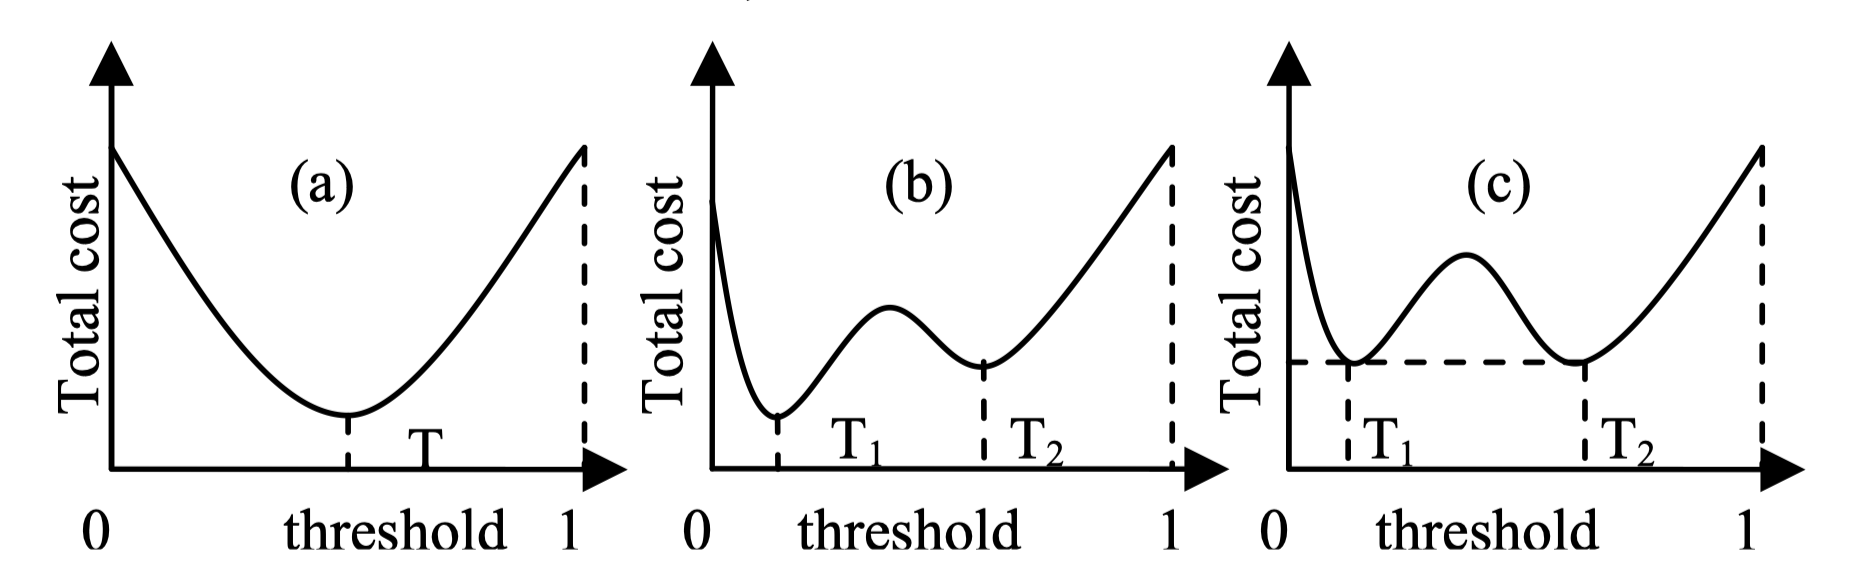
\includegraphics[width=0.6\textwidth]{slides/imbalanced-learning/figure/threshold_adjusting.png}
        \end{figure}

        \item The optimal threshold $T^{*}$ corresponds to the point with the smallest $M_C$.

        \item What if two local minima? We prefer the one whose ``valley'' has a wider span (e.g. $T_2$ in the 3rd subfigure). Because it is less sensitive to small changes in $T$.

        \item Search the best $T$ on \textbf{validation} sets, and do $K$-fold cross-validation to avoid overfitting!
    \end{itemize}
\end{vbframe}

\begin{vbframe}{MetaCost: Overview}

	\small{
	\begin{itemize}

		\item In stead of making individual algorithms cost-sensitive, a better solution would be converting cost-insensitive classifiers into cost-sensitive ones.

		\item MetaCost is a wrapper method:
        \begin{itemize}
            \small
            \item can be used for \emph{any} type of classifier to obtain a cost-sensitive classifier.
            \vspace{5pt}
            
            \item treats underlying classifier as a black-box, $\leadsto$ no knowledge about its mechanism is required, and no changes to its mechanism is needed.
            \vspace{5pt}
            
            \item needs only a cost-matrix $\mathbf{C}$, which is used to adapt the decision boundaries. {\scriptsize (Some tuning parameters are also needed.)}
            \vspace{5pt}
            
            \item The rough procedure: 
                \begin{enumerate}
                    \small
                    \item relabel the training examples with their ``optimal'' classes, i.e., the ones with low expected costs;
                    \vspace{5pt}
                    
                    \item apply the classifier on the relabeled data set.
                \end{enumerate} 
        \end{itemize}

	\end{itemize}

	}

\end{vbframe}


\begin{vbframe}{MetaCost: Algorithm}
	
	\scriptsize{
%		
 	The procedure of MetaCost is divided into three phases:
			%			
		\begin{minipage}{0.53\textwidth} 
%				
				\begin{enumerate}
%					
					\scriptsize
					\item Bagging --- The underlying classifier is used (trained) $L$ times on different bootstrapped samples of the training data, respectively.
%					
					\item Relabeling --- These $L$ trained classifiers are used to relabel the original training data set by taking the cost-matrix into account.
%					
					\item Cost-sensitivity ---  The classifier is trained on the relabeled data set resulting in a cost-sensitive classifier.
%					
				\end{enumerate}
%
	\scriptsize
	\lz 
			Predictions of the classifier $f$ are converted (if necessary) into probabilistic prediction:
			\begin{center}
				\tiny
							ProbPrediction$(j,f,\xv) = \begin{cases}
					(f(\xv))_j & \mbox{$f$ is a prob.\ classifier,} \\
					\mbox{One-hot$(f(\xv))$}& \mbox{else,}
				\end{cases}$
			\end{center}
%		
		\scriptsize
		where One-hot$(f(\xv))$ uses a one-hot-encoding of the prediction to make it a probability. 
		
		\end{minipage}
		\begin{minipage}{0.45\textwidth} 
			\begin{algorithmic}
				
				\tiny
%				
				\State \textbf{MetaCost}  
				\State \textbf{Input:} 
				$\D = \{(\xi,\yi)\}_{i=1}^n$ training data, \\
				$L \in \N$ number of bagging iterations, \\
				$B \in \N$ bootstrap size, \\
				$f$ (black-box) classifier, 
				$\mathbf{C}$ cost matrix, 
%				$g = |\Yspace|$ number of classes
				\State \# 1st phase:
				\For{$l=1,\ldots,L$}
					\State $\D_l  \leftarrow $ BootstrapSample ($\D,B$)
					\State $f_l  \leftarrow $ train $f$ on $\D_l$
				\EndFor
				\State \# 2nd phase:
				\For{$i=1,\ldots,n$}
					\If{$\xi \in \D_l$ for all $l=1,\ldots,L$}
						\State $\tilde L \leftarrow \{1,\ldots,L\}$
					\Else
						\State $\tilde L \leftarrow \bigcup_{l: \xi \notin \D_l} \{l\}$
					\EndIf
					\For{$j=1,\ldots,g$} (relabel for binary case)
						\State $p_j(\xi)  \leftarrow \frac{1}{|\tilde L| } \sum_{l \in \tilde L}   p_j(\xi~|~ f_l) $
						\State $p_j(\xi~|~ f_l) = $ ProbPrediction$(j,f_l,\xi)$
						\State $\tilde y^{(i)} \leftarrow \argmin_{i^*} \sum_{j=1}^g p_j(\xi) C(i^*,j) $
					\EndFor
					\State $\tilde D \leftarrow \tilde D \cup \{(\xi,\tilde y^{(i)})\} $
				\EndFor
				\State \# 3rd phase:
%				
				\State $f_{meta} \leftarrow$ train $f$ on $\tilde D$
%			
			\end{algorithmic}
		\end{minipage}
		%
	}
	%	
\end{vbframe}

%%%%%



%%%


%\begin{vbframe}{MetaCost: Example}
%	%	
%	\small{
%		\begin{itemize}
%			%		
%			\item We compare C4.5 (decision tree) with MetaCost using C4.5 for the \href{http://staffwww.itn.liu.se/~aidvi/courses/06/dm/
%				labs/heart-c.arff}{heart data set}  in \href{ http://www.cs.waikato.ac.nz/ml/weka/}{Weka}. 
%			%		
%			\item The cost matrix $\mathbf{C}$ is 
%			
%			\begin{center}
%				\begin{tabular}{cc|cc}
%					& &\multicolumn{2}{c}{True class} \\
%					& & $y=1$ & $y=-1$  \\
%					\hline
%					\multirow{2}{*}{\parbox{0.3cm}{Pred.  class}}& $\hat y$ = 1     & $0$                & $ 1 $\\
%					& $\hat y$ = -1 & $ 4 $              &  $0$   \\
%				\end{tabular}
%			\end{center}
%		
%			\item The resulting confusion matrices are 
%			
%						
%			\begin{center}
%				\begin{tabular}{cc|cc}
%					& &\multicolumn{2}{c}{True class} \\
%					& MetaCost & $y=1$ & $y=-1$  \\
%					\hline
%					\multirow{2}{*}{\parbox{0.3cm}{Pred.  class}}& $\hat y$ = 1     & $104$                & $ 21 $\\
%					& $\hat y$ = -1 & $ 61 $              &  $117$   \\
%				\end{tabular}
%							\begin{tabular}{cc|cc}
%				& &\multicolumn{2}{c}{True class} \\
%				& C4.5 & $y=1$ & $y=-1$  \\
%				\hline
%				\multirow{2}{*}{\parbox{0.3cm}{Pred.  class}}& $\hat y$ = 1     & $138$                & $ 40 $\\
%				& $\hat y$ = -1 & $ 27$              &  $98$   \\
%			\end{tabular}
%			\end{center}
%		
%		
%			%		
%			\item The total cost of MetaCost is 145, while C4.5 has total costs of 187. However, MetaCost has $0.729$ correct classifications and C4.5 has $0.779.$ 
%			
%			%		
%		\end{itemize}
%		%
%	}
%	%	
%\end{vbframe}



%\begin{vbframe}{Cost-Sensitive Decision Trees}
%	%	
%	\small{
%		\begin{itemize}
%			%		
%			\item 
%			%		
%		\end{itemize}
%		%
%	}
%	%	
%\end{vbframe}


%
\endlecture
\end{document}
